\subsection{Reinforcement Learning Model}

The basic model used in our intelligent antenna alignment framework consists of a
lightweight reinforcement learning (RL) algorithm designed to learn the optimal
orientation of the receiver antenna by maximizing the received signal strength.
Unlike the typical model-based control approaches, RL allows us to learn a useful
control policy without using any channel model information.

\subsubsection{Overview of Reinforcement Learning Framework}

Reinforcement learning is a kind of learning approach whereby an intelligent agent
learns how to take actions to maximize total cumulative rewards in a given
environment. In contrast to supervised learning, which assumes the knowledge of the
input-output mappings, RL only involves scalar feedbacks telling the agent whether it
has done something well or not. The RL framework is highly appropriate for
controlling systems with no available models~\cite{ref19}.

\begin{figure}[H]
    \vspace{1em} 
    \centering
    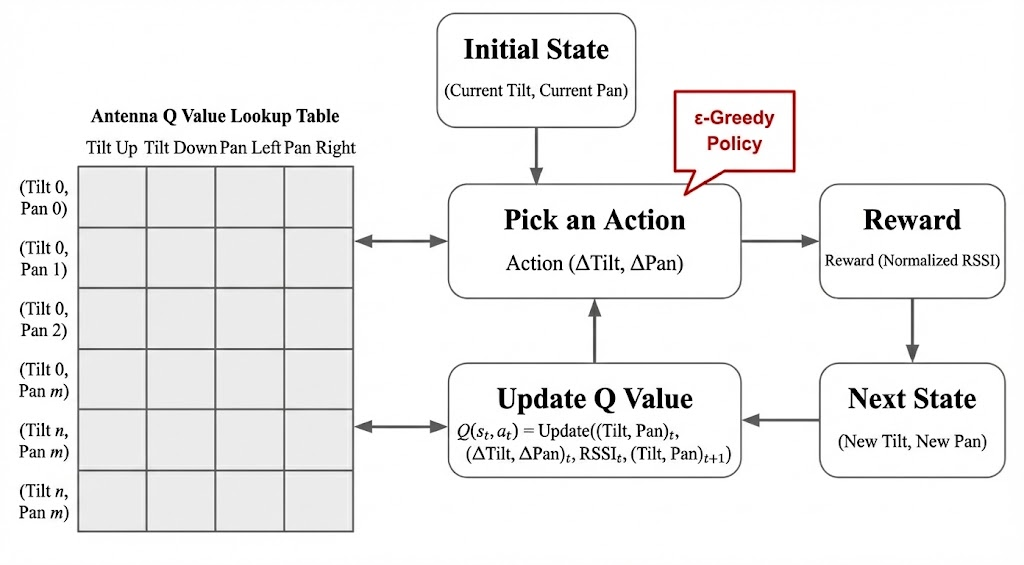
\includegraphics[width=1\textwidth]{images/rl_flow.png}
    \caption{Reinforcement Learning Process Flow}
    \label{fig:rl_flow}
\end{figure}

Model-free reinforcement learning algorithms, such as Q-learning, approximate the
expected long-term return of taking a particular action at a state without modeling
the environment dynamics explicitly. This approach is promising for our case study,
as the resulting controller should execute on a resource-constrained platform that has
deterministic runtime requirements. Here, learning is done off-line, while only the learned
Q-table is uploaded onto the device.

\subsubsection{Q-Learning}

Q-learning was chosen due to its favorable trade-off of learning capacity, implementation
simplicity, and embedded feasibility in this scenario. Antenna alignment is formulated as a
task with a small state-action space and runs deterministically in terms of memory usage
and compute requirements, therefore the tabular variant of Q-learning is an optimal choice.
The algorithm learns a policy off-line, after which it can be applied as a simple fixed-size
lookup table with very low latency.

The alternative SARSA was ruled out, since it is an on-policy algorithm, and hence its
learning relies on the same exploratory policy. On-policy learners are known to yield more
conservative results, which is a nice property in some safety-sensitive applications.
However, in the present scenario, we wanted to learn a strong greedy policy and apply it
deterministically on hardware. Thus, Q-learning is more aligned with our aims, as it
directly optimizes a greedy policy's values.

Finally, Deep Q-Networks were not considered, since their strengths manifest themselves
in cases where the state space is relatively large or continuous. However, in this project,
the state space was intentionally kept small via discretization, so the application of a
neural network-based DQN algorithm would require additional training complexity,
hyperparameter tuning, and increased deployment costs.

The model is cast as a Markov Decision Problem (MDP) that consists of:
\begin{itemize}
    \item \textbf{State ($s_t$):} The state space comprises the present azimuth,
    tilt indices, and RSSI trend classification.
    \item \textbf{Action ($a_t$):} The actions space includes discrete movements
    such as panning left, panning right, tilting up, tilting down, and holding the position.
    \item \textbf{Reward ($r_t$):} The scalar reward denotes the variation in
    averaged RSSI from the action, along with a minor cost for movement.
    \item \textbf{Policy:} An $\epsilon$-greedy strategy explores and exploits in
    the learning process. A greedy strategy is adopted at inference time.
\end{itemize}

\subsubsection{Exploration--Exploitation Balance}

In the training process, the reinforcement learning agent uses an $\epsilon$-greedy approach
to first explore the problem space and then use it to exploit what it learns from its past
experiences. Initially, exploration rate needs to be large, since the agent has to go through
favorable and unfavorable states in terms of the antenna position in order to form an
appropriate Q-table and not just optimize from few positions that it starts from.

During the learning process, the exploration factor is slowly decayed, allowing more exploitation.
Decay was appropriate in this case because after sampling the space adequately, further
exploration would lead to increased convergence time. In other words, once the space was
sufficiently explored, further exploration served only the purpose of adding unnecessary noise
to the learning process and slowing the convergence of Q-values. Exploration rate drops
to zero during deployment for repeatability purposes.

\subsubsection{Learning Convergence}

Convergence in our context means convergence of the Q-table values together with the
corresponding trend toward improved performance of the algorithm. From a practical point
of view, convergence could be defined as the point at which the reward-per-episode curve,
as well as RSSI improvement, stops increasing significantly and the policy reaches favorable
states in diverse scenarios. In other words, the point of convergence corresponds to the
situation when the improvement of the performance does not show clear trends anymore.

This approach was appropriate in our case due to the fact that the goal was to develop an
effective deployment policy, not to prove an optimal solution to the underlying problem in
the abstract Markov Decision Process.

\subsubsection{Q-Learning Algorithm Pseudocode}

The below pseudocode summarizes the adopted Q-learning training and deployment procedure that was used.

\begin{minted}[linenos, fontsize=\small]{c}
# Initialize Q-table
init Q[s, a] for all states s and actions a
set alph (learning rate), gamma (discount factor), 
epsilon (exploration rate)

for each episode:
    reset env. to a valid random initial orientation
    
    measure averaged RSSI
    encode current state s

    for each step until terminal condition or max_steps:
        
        # Action selection (epsilon-greedy)
        with probability epsilon:
            choose a random action a
        else:
            choose a = argmax_a Q[s, a]

        # Apply action
        apply action a
        
        measure next averaged RSSI
        compute reward r from RSSI change and movement penalty
        
        encode next state s_next

        # Q-learning update
        Q[s, a] = Q[s, a] + alpha * (
            r + gamma * max_a' Q[s_next, a'] - Q[s, a]
        )

        s = s_next

    # Exploration decay
    decay epsilon

# Export trained model
export converged Q-table to ESP32-S3 firmware

# Deployment (inference only)
during deployment:
    choose a = argmax_a Q[s, a]
    do not perform online learning
\end{minted}


\subsubsection{Design of State Space}
The state space contains all the information that is accessible to the RL agent in
every decision-making step. In order to ensure a compact design of the state space,
the implemented controller utilizes only practical limitations of movement of the
hardware instead of a $360^{\circ}$ rotation:
\begin{itemize}
    \item Discretization of the azimuth angle into $N_\theta = 19$ states
    within the range $0^{\circ}$-$180^{\circ}$ with $10^{\circ}$ increment
    \item Discretization of the tilt angle into $N_\phi = 11$ states
    within the range $25^{\circ}$-$75^{\circ}$ with $5^{\circ}$ increment
    \item Classification of RSSI change into $N_r = 3$ categories: ascending,
    constant, and descending
\end{itemize}
Thus, the resulting state is defined as the combination of the indexes of the
azimuth, tilt angles, and RSSI change:
\begin{equation}
s_t = \left(i_{\theta},\, i_{\phi},\, i_r \right)
\end{equation}
The number of possible states is equal to:
\begin{equation}
\left|S\right| = N_\theta \times N_\phi \times N_r = 19 \times 11 \times 3 = 627
\end{equation}


\subsubsection{Size of the Q-Table and Storage Requirement}

Q-table size is a function of the number of discrete state and action spaces. Assume
that the pan (azimuth) angle takes on $N_\theta$ positions and that the tilt
(elevation) angle takes on $N_\phi$ positions. Further, assume that there are $N_r$
discrete values for RSSI trends and $N_a$ actions available. The size of the
Q-table is:
\begin{equation}
\left|Q\right| = N_\theta \times N_\phi \times N_r \times N_a
\end{equation}

In the case of the deployed controller:
\begin{itemize}
    \item Pan states: $N_\theta = 19$
    \item Tilt states: $N_\phi = 11$
    \item RSSI trend states: $N_r = 3$
    \item Actions: $N_a = 5$ (left, right, up, down, hold)
\end{itemize}

Hence, the deployed table contains:
\begin{equation}
\left|Q\right| = 19 \times 11 \times 3 \times 5 = 3,135 \text{ Q-values}
\end{equation}
Assuming each Q-value is stored as a 32-bit floating-point number (4 bytes), the
memory requirement is:
\begin{equation}
3,135 \times 4~\text{bytes} \approx 12.3~\text{kB}
\end{equation}
This memory footprint is comfortably within the RAM capacity available on the
ESP32-S3, confirming the feasibility of direct on-device inference.

\subsubsection{Action Space Design}
The action space comprises the available movement possibilities for the antenna
that can be taken by the RL agent. The actions are defined as discrete values
corresponding directly to the actual actuator commands.

\begin{itemize}
    \item \textbf{Pan left}: decrease azimuth by one $10^{\circ}$ step
    \item \textbf{Pan right}: increase azimuth by one $10^{\circ}$ step
    \item \textbf{Tilt up}: increase tilt by one $5^{\circ}$ step
    \item \textbf{Tilt down}: decrease tilt by one $5^{\circ}$ step
    \item \textbf{Hold}: retain the current orientation
\end{itemize}

Pan actions are performed using the stepper motor controller, whereas tilt actions
are performed using the servo output signal. The discrete nature of the action
space simplifies the inference process.

\subsubsection{Reward Function}
The reward function gives feedback to the reinforcement learning algorithm
by assessing the effect of each antenna motion on link quality. In particular,
the aim is to maximize RSSI without making any unnecessary movements that might cause oscillation, wear, or delay in convergence.

The instantaneous reward at time step $t$ is defined as:
\begin{equation}
r_t = \Delta RSSI_t - \lambda \cdot \mathbb{I}_{\text{move}}
\end{equation}
where:
\begin{itemize}
    \item $\Delta RSSI_t$ is the change in averaged RSSI after executing the action
    \item $\mathbb{I}_{\text{move}}$ is equal to $1$ when a physical movement occurs
    and $0$ for the hold action
    \item $\lambda$ is a weighting factor that penalizes unnecessary actuation
\end{itemize}

In this way, when the action leads to an increase in RSSI, there will be a positive reward. On the other hand, negative rewards will follow in case the action leads to a decrease in RSSI values, which makes the learning algorithm move towards optimal positions for antenna. Lastly, the motion penalty ensures that the antenna movements do not take place unnecessarily.

Parameter $\lambda$ is empirically chosen such that the reward always consists mainly of RSSI increases rather than any unnecessary antenna movements.

\subsubsection{Learning and Action Selection}

In the process of performing actions, the agent utilizes the pre-trained Q-table 
on the MCU. The Q-table was pre-computed offline in the simulator based on multiple 
episodes with varying initial states in terms of orientation angles.

\textbf{Actions Selection:} 
The agent decides its action according to Q-values that were obtained previously:
\begin{equation}
a_t = \arg\max_a Q(s_t, a)
\end{equation}
Here $s_t$ is the current state described by orientation index values and RSSI change trend.

There was no exploration applied during deployment so that hardware trials remain stable,
repeatable, and comparable across runs.

\subsubsection{Implementation Considerations for ESP32-S3}

\begin{itemize}
    \item \textbf{Memory usage:} The Q-table size is about
    $12.3$~kB and can be allocated statically
    \item \textbf{Computational overhead:} Action determination involves just table
    lookup and arithmetic operations
    \item \textbf{Real-time performance:} ESP32-S3 constantly monitors RSSI, extracts
    the state code, selects the optimal action, and controls actuators
    \item \textbf{System stability:} As there is no learning phase, the solution does
    not experience drift from trial to trial
\end{itemize}

In conclusion, the presented design makes the antenna adjustment procedure fully automated and sensitive to environmental changes while being easy to implement as an embedded solution.